\section{Onboarding cost across 8 robots}
\label{sec:onboarding}

\begin{figure*}[t]
\centering
\setlength{\tabcolsep}{1pt}
\renewcommand{\arraystretch}{0.4}
\begin{tabular}{cccccccc}
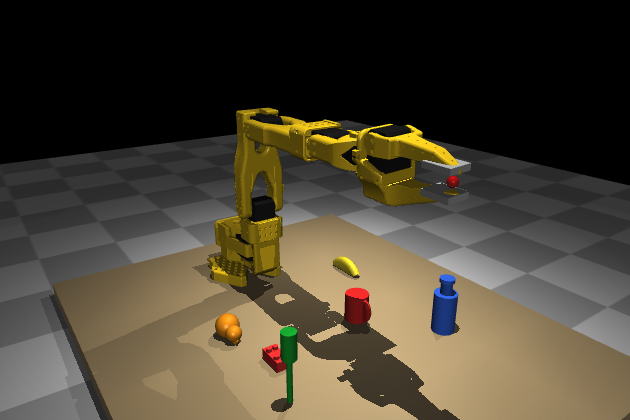
\includegraphics[width=0.118\textwidth]{figures/zoo_so101.png} &
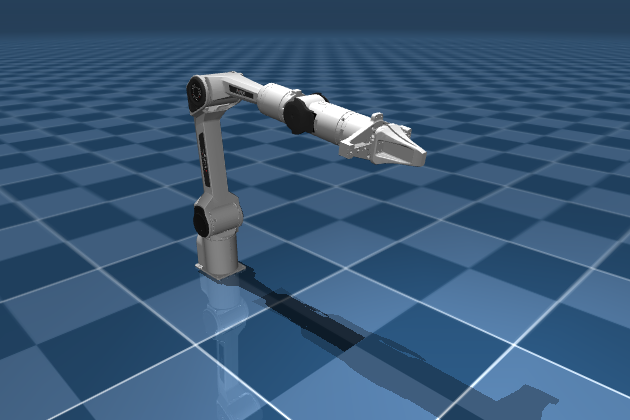
\includegraphics[width=0.118\textwidth]{figures/zoo_piper.png} &
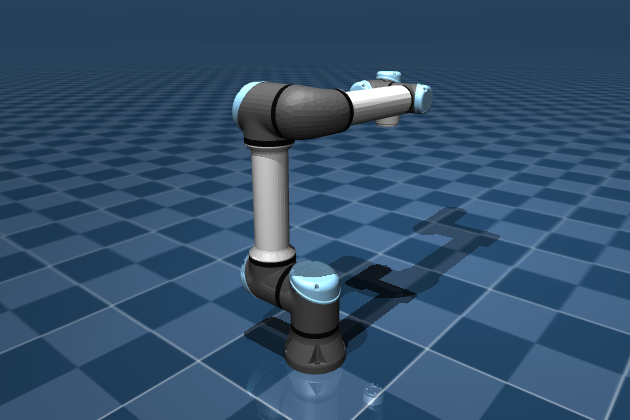
\includegraphics[width=0.118\textwidth]{figures/zoo_ur5e.png} &
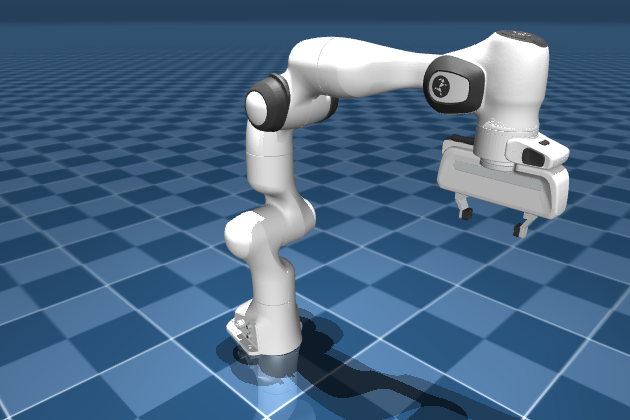
\includegraphics[width=0.118\textwidth]{figures/zoo_franka.png} &
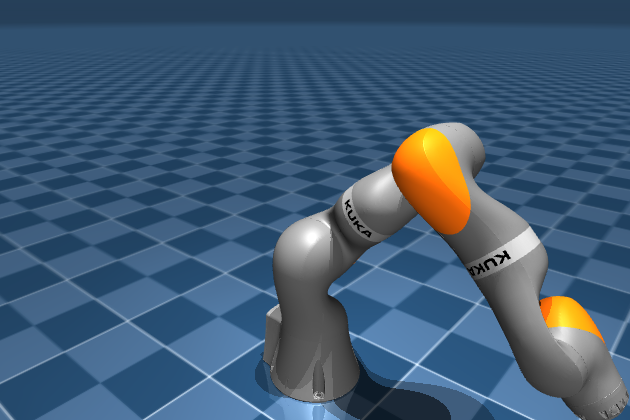
\includegraphics[width=0.118\textwidth]{figures/zoo_kuka.png} &
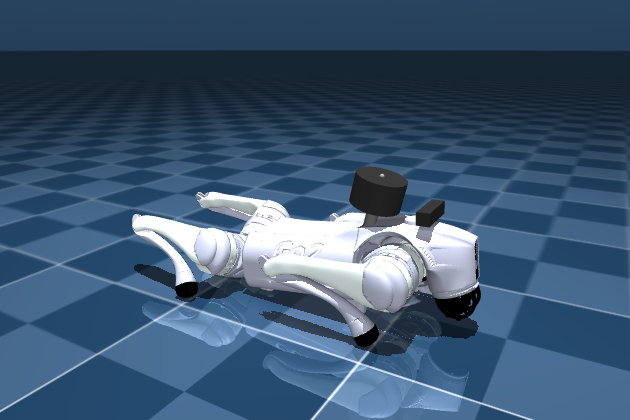
\includegraphics[width=0.118\textwidth]{figures/zoo_go2.png} &
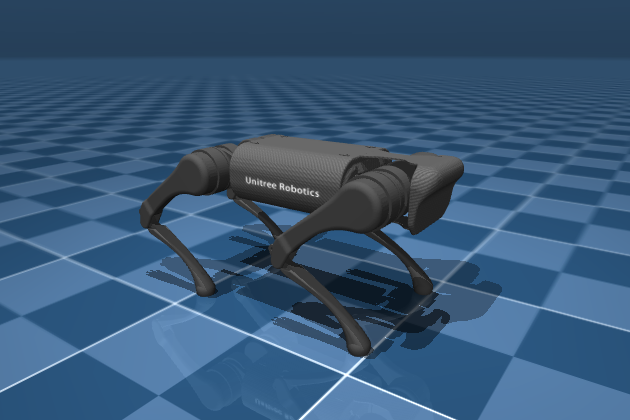
\includegraphics[width=0.118\textwidth]{figures/zoo_a1.png} &
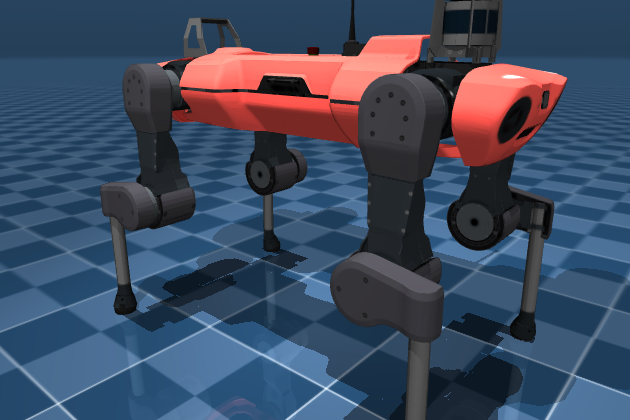
\includegraphics[width=0.118\textwidth]{figures/zoo_anymal.png} \\
{\tiny SO-101 (5)} & {\tiny Piper (6)} & {\tiny UR5e (6)} &
{\tiny Franka (7)} & {\tiny KUKA (7)} & {\tiny Go2 (12)} &
{\tiny A1 (12)} & {\tiny ANYmal-C (12)} \\
{\tiny 5.1\,min} & {\tiny 6.4\,min} & {\tiny 6.8\,min} &
{\tiny 8.4\,min} & {\tiny 8.0\,min} & {\tiny 9.1\,min} &
{\tiny 8.6\,min} & {\tiny 10.0\,min} \\
\end{tabular}

\vspace{4pt}

\setlength{\tabcolsep}{1pt}
\renewcommand{\arraystretch}{0.3}
\begin{tabular}{ccccc}
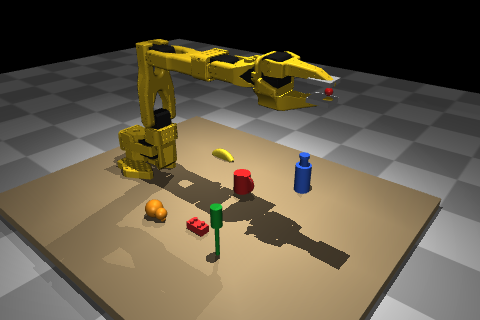
\includegraphics[width=0.18\textwidth]{figures/film_swap_0.png} &
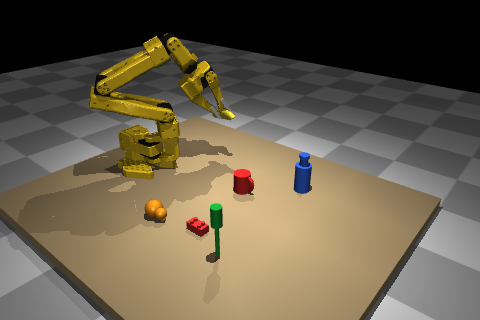
\includegraphics[width=0.18\textwidth]{figures/film_swap_1.png} &
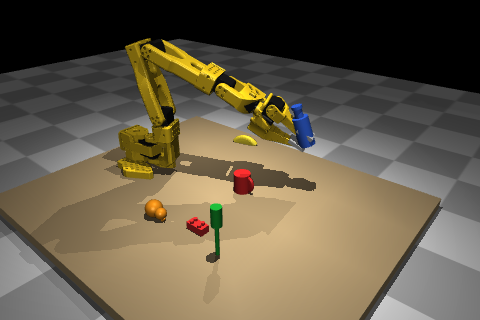
\includegraphics[width=0.18\textwidth]{figures/film_swap_2.png} &
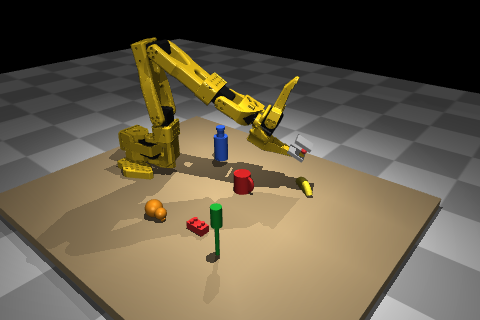
\includegraphics[width=0.18\textwidth]{figures/film_swap_3.png} &
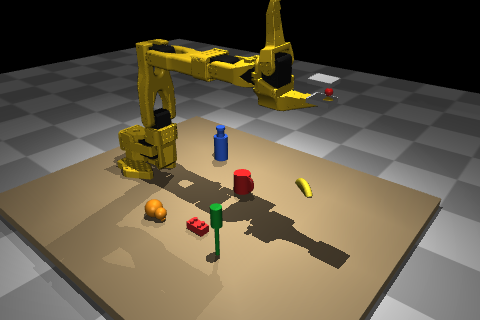
\includegraphics[width=0.18\textwidth]{figures/film_swap_4.png} \\
\multicolumn{5}{c}{\parbox{0.92\textwidth}{\centering\scriptsize\textbf{(a) SO-101
\texttt{swap\_banana\_bottle}} (contact-rich hard suite, \S\ref{sec:cap-portability}):
pick banana $\rightarrow$ park $\rightarrow$ relocate bottle
$\rightarrow$ banana to bottle's origin; weld-grasp driver, $5/5$.}} \\[3pt]
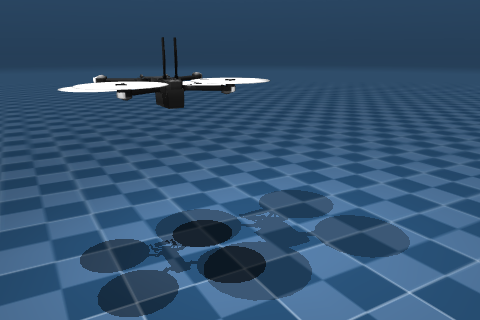
\includegraphics[width=0.18\textwidth]{figures/film_patrol_0.png} &
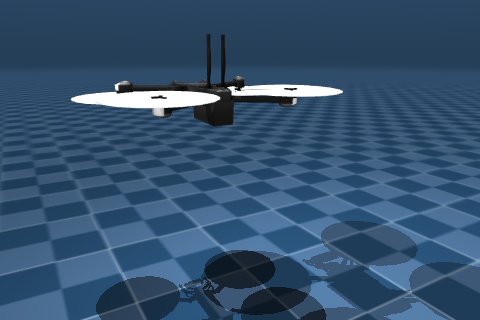
\includegraphics[width=0.18\textwidth]{figures/film_patrol_1.png} &
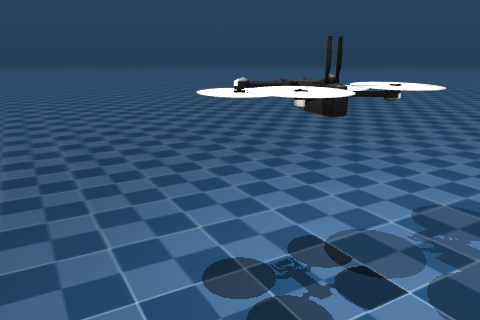
\includegraphics[width=0.18\textwidth]{figures/film_patrol_2.png} &
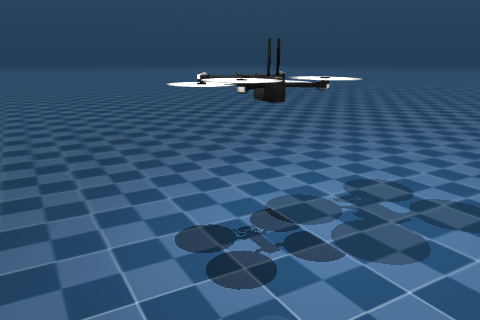
\includegraphics[width=0.18\textwidth]{figures/film_patrol_3.png} &
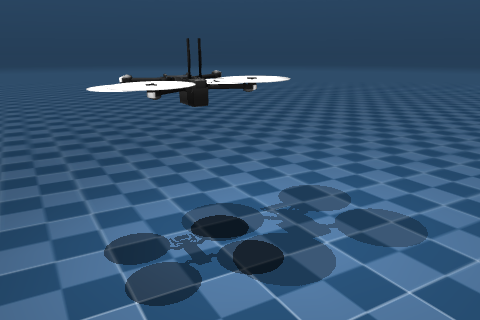
\includegraphics[width=0.18\textwidth]{figures/film_patrol_4.png} \\
\multicolumn{5}{c}{\parbox{0.92\textwidth}{\centering\scriptsize\textbf{(b) Skydio~X2
\texttt{box\_patrol}} (appendix-only aerial suite, Appendix~\ref{app:morphology}): takeoff to
0.6\,m, then a 0.4\,m square via four corners (waypoint tolerance
0.18\,m); synthesized cascaded thrust controller, $5/5$.}} \\
\end{tabular}
\caption{\textbf{Top:} the eight target robots (synthesis
wall-clock beneath each; no per-robot tuning), one prompt each at
\$$2.98 \pm \$0.84$, $7.8 \pm 1.6$\,min (\S\ref{sec:onboarding}).
\textbf{Bottom:} synthesized drivers running an SO-101 object-swap
(a) and a Skydio~X2 patrol (b); more in
Appendix~\ref{app:filmstrips}--\ref{app:gallery}.}
\label{fig:hero}
\end{figure*}


Running the pipeline once on each of the eight robots in
Figure~\ref{fig:hero} (top) gives 8/8 structural-validation pass;
under the released strict harness 0/8 \emph{fully} pass (arms: a
post-synthesis perception check; quadrupeds: locomotion tests;
Appendix~\ref{app:onboarding}). Mean
wall-clock time is $7.8 \pm 1.6$ minutes (5.1\,min on SO-101 to
10.0\,min on ANYmal-C) and mean LLM-inference cost is
$\$2.98 \pm \$0.84$ per robot ($\$23.80$ and 62\,min total).

These numbers are in self-contained mode (\S\ref{sec:modes})
with bounded per-phase iteration caps. Validation
per robot covers five shared steps: no-skeleton import, robot-class
check, driver build, \texttt{home()} settling, and a \texttt{describe} check. It
then runs an IK round-trip and \texttt{gripper\_cycle} on arms, or
\texttt{stand\_up}/\texttt{sit}/\texttt{walk\_forward} on quadrupeds.
\emph{Practitioner takeaway: structural onboarding of a new MJCF
costs ${\approx}\$3$ and ${\approx}8$ minutes of LLM time, before
any human driver engineering.}
